% This is copied from 2017 ESF and it is example of LaTex
% -------------------------------------------------------
% Ondřej Šereda 8.2.2018

\subsubsection{Description/concept}
\iffalse
Describe your concept of the shutdown circuit, the master switches, shut down buttons, brake over travel switch, etc.
Additionally, fill out the following table replacing the values with your specification and append additional switches from your setup:
\fi

Shutdown circuit (SDC) starts in ECUP unit, then goes through all SDC elements in the car and ends in ECUA, which is placed inside the Accumulator Pack. In ECUP SDC starts from LV power +24V and ends in ACP by powering AIR coils switching circuit (See \ref{fig:SDC-scheme}). The SDC consists of 2 master switches, 3 shut-down buttons(SDB), the brake-over-travel-switch(BOTS), the insulation monitoring device (IMD), the inertia switch, the brake system plausibility device(BSPD), interlocks in Motor Controllers and Accumulator Pack and the accumulator management system (AMS). All of these crucial parts do not act through any power stage, but carry directly the AIR current.

\begin{figure}[H]
	\includegraphics[width=\textwidth, trim={2cm 3cm 2cm 2cm},clip]{./img/sdc-scheme.pdf}
	\caption{SDC scheme.}
	\label{fig:SDC-scheme}
\end{figure}

\begin{table}[H]
	\caption{List of switches in the shutdown circuit}
	\centering
	\begin{tabularx}{\textwidth}{|X|l|}
		\hline Part  & Function \\[\TableSize]
		\hline Main Switch (for control and tractive-system; CSMS, TSMS) & Normally open \\[\TableSize]
		\hline Brake over travel switch (BOTS) & Normally closed \\[\TableSize]
		\hline Shutdown buttons (SDB) & Normally closed \\[\TableSize]
		\hline Insulation Monitoring Device (IMD) & Normally open \\[\TableSize]
		\hline Battery Management System (BMS) & Normally open \\[\TableSize]
		\hline Inertia Switch & Normally closed \\[\TableSize]
		\hline Interlocks & Closed when circuits are connected \\[\TableSize]
		\hline Brake System Plausibility Device & Normally Open \\[\TableSize]
		\hline
	\end{tabularx}%
	\label{tab:SDCswitch}%
\end{table}%


\paragraph{Monitoring SDC}
Every part of SDC is monitored by specific ECU (Electronic Control Unit) in order to identify disconnected element. BOTS is measured by ECUP, SDB-center  and Inertia switch are measured by ECUF , interlocks in Motor Controllers are measured by Motor Controllers, Interlock in Accumulator Pack is measured by ECUA  and finally SDB-right, SDB-left and TSMS   are measured by ECUB. Every piece of information regarding the state of closure SDC are running between ECU´s by CAN. 

We designed SDC to be ‘single wire’ alike and distanced it from the system as much as it was possible. In order to remain SDC as a stand-alone wire we used optocouplers for main points of SDC. Optocouplers are connected in such a way, that they become active only in case of nonzero voltage occurance at a certain point of SDC.

ECUB monitors the last poit of SDC (behind TSMS). If a state of error od SDC is detected ECUB latches the off-state of SDC to stay off. If the ocured error is non-critical, it allows pilot to re-enter the TSON state. If monitored error is criticall (such as IMD etc.), it notes the error to the memory-storrage and does not allow SDC to become active until appropriate steps are taken. The logic flow-chart is shown in \ref{ECUA-Jansixta}. For more info about this look to next and \nameref{subsec:Reset} sections. SDC error states that require special handling

\ref{Jan sixta}
ECUB is last part of SDC before TSMS. It implements latching function using external memory so even in case of total shutdown of LV power it is possible to remember error states that occurred before the breakdown. The ECUB implements enough capacitor storrage, that it is able to write the error to the memory even in case of imidiate power-loss cased by the error. It is not possible to reactivate SDC and close AIRs until all the steps required by rules are done.

\paragraph{Master Switch}
We use Autolec Mini-Master battery cut-out switches with continuous current rating 100A, shown on \ref{fig:SDC-TSMS}.
\begin{figure}[H]
	\centering
	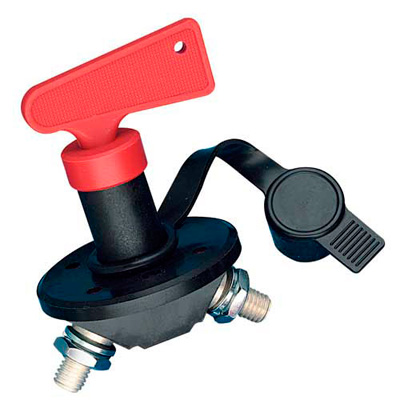
\includegraphics[width=.5\textwidth]{./img/SDC-TSMS.jpg}
	\caption{TSMS.}
	\label{fig:SDC-TSMS}
\end{figure}

\paragraph{Shutdown Switch}
We use OMRON A165E shutdown buttons, which have 3A current rating at 30VDC.

On the cockpit it is OMRON A165E-LS, shown on \ref{fig:SDC-A165E-LS}.
\begin{figure}[H]
	\centering
	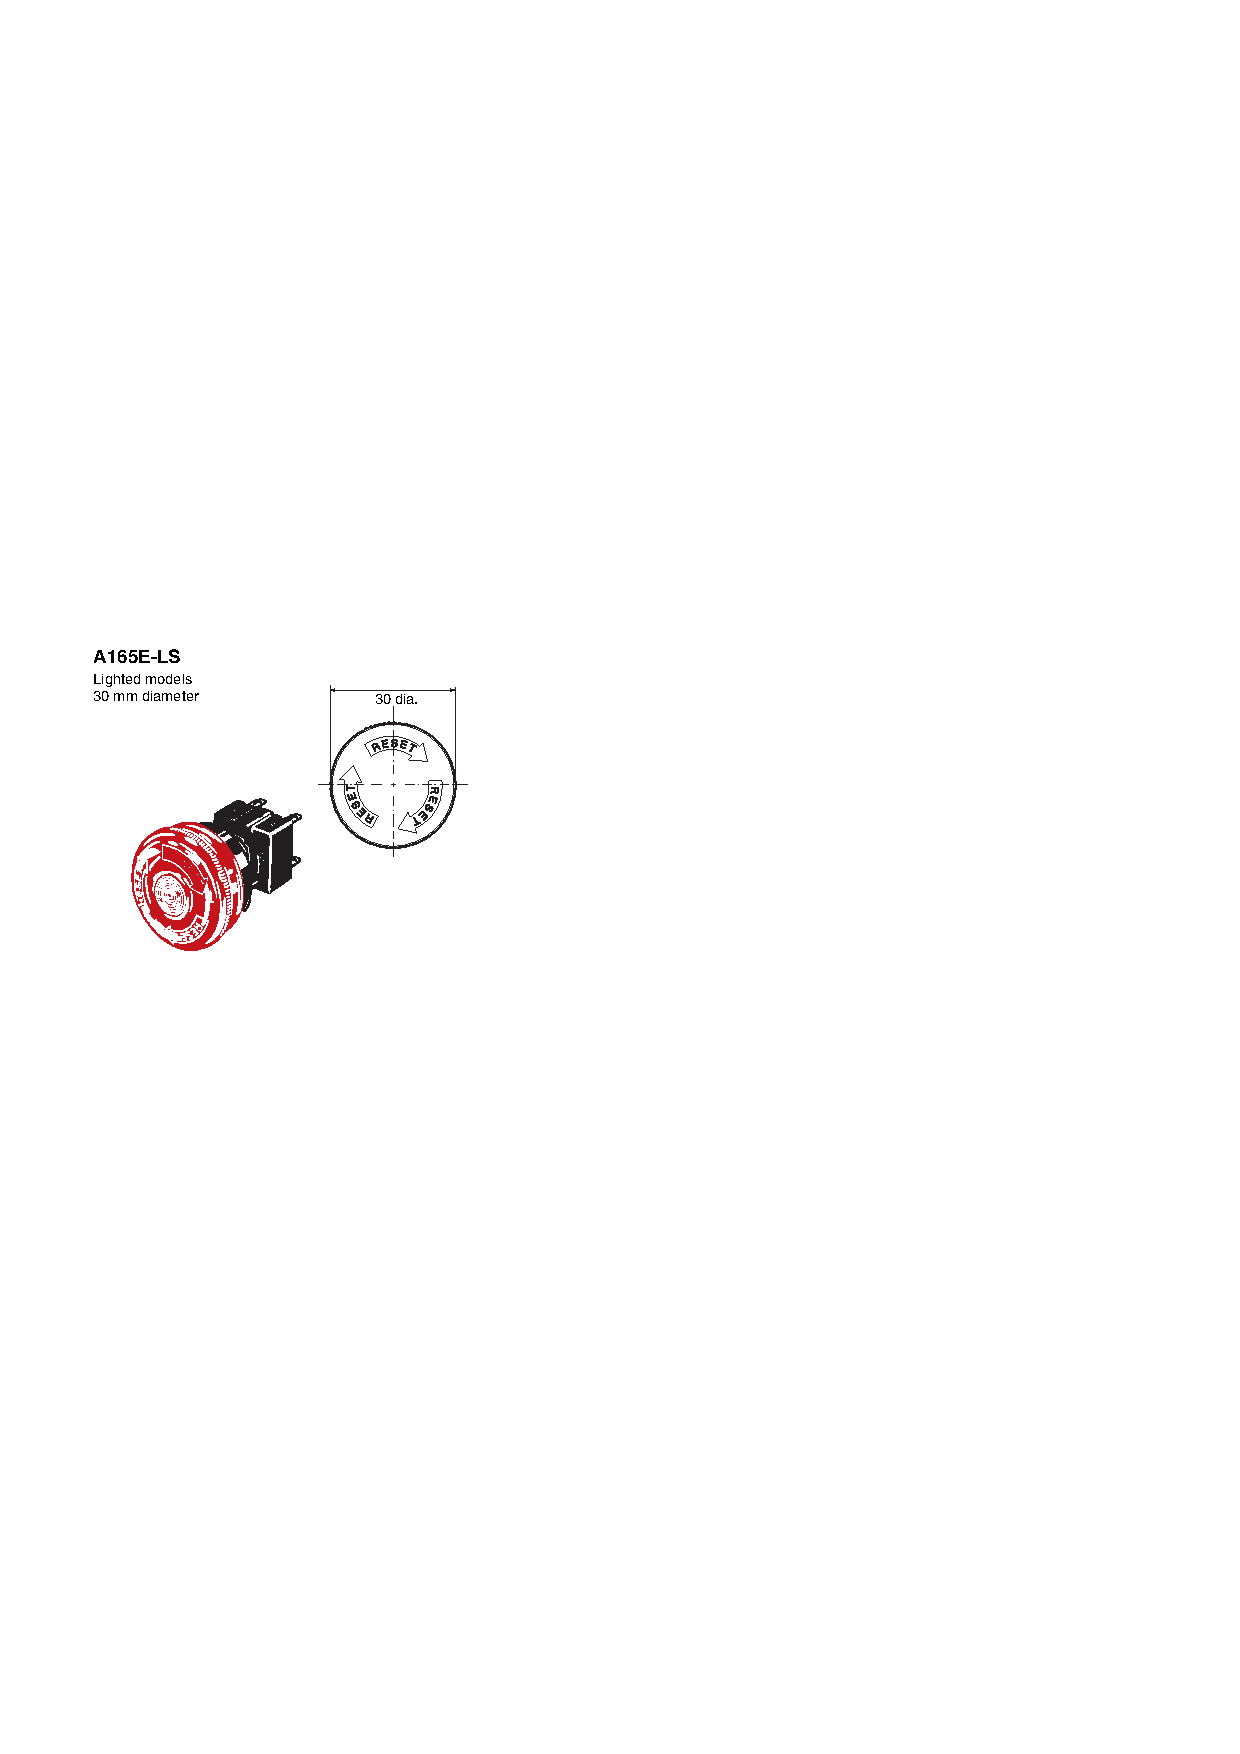
\includegraphics[width=.5\textwidth]{./img/SDC-A165E-LS.pdf}
	\caption{Cockpit SDB.}
	\label{fig:SDC-A165E-LS}
\end{figure}

On the left and on the right sides there are OMRON A165E-LM buttons, shown on \ref{fig:SDC-A165E-LM}.
\begin{figure}[H]
	\centering
	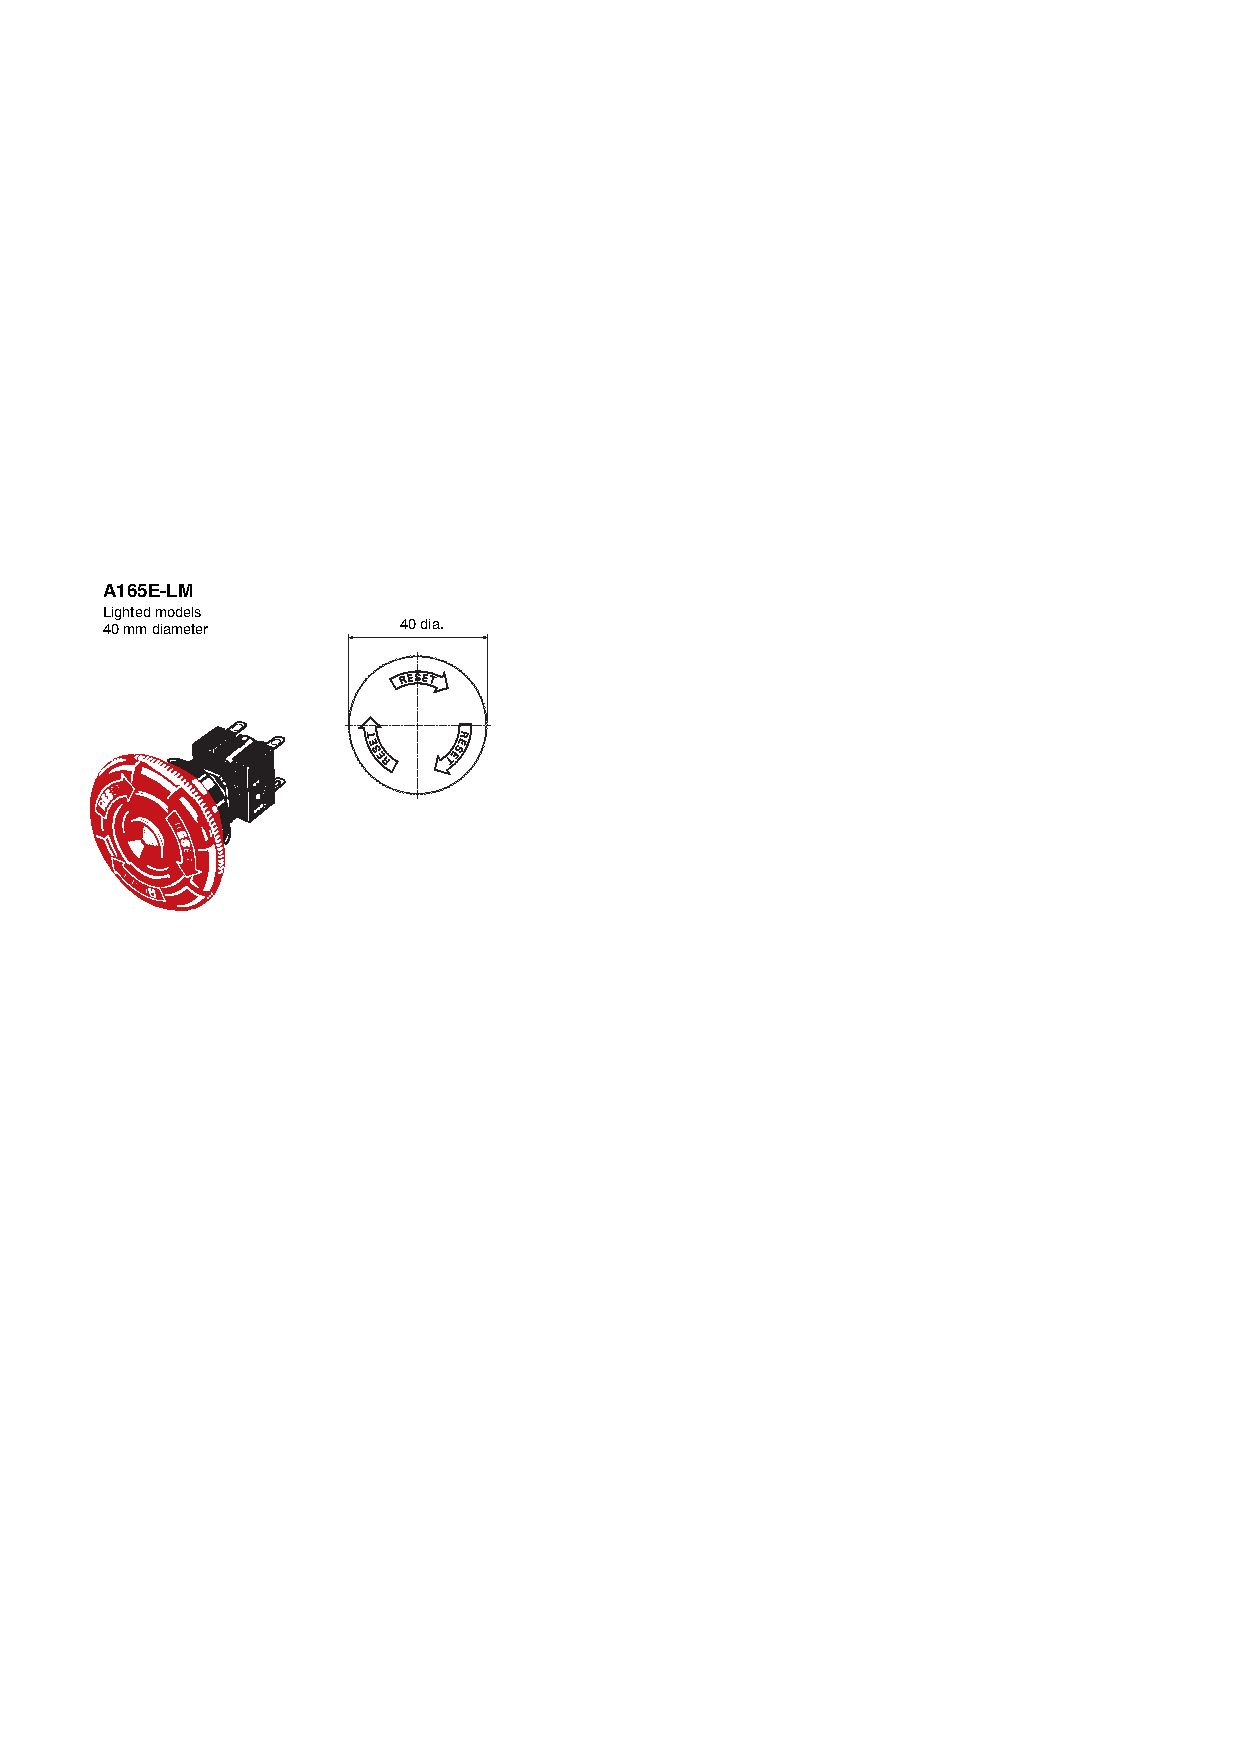
\includegraphics[width=.5\textwidth]{./img/SDC-A165E-LM.pdf}
	\caption{SDB left and right.}
	\label{fig:SDC-A165E-LM}
\end{figure}

\paragraph{Brake Over Travel Switch}
It is type A165E-M, current raging 3A, shown on \ref{fig:SDC-A165E-M}
\begin{figure}[H]
	\centering
	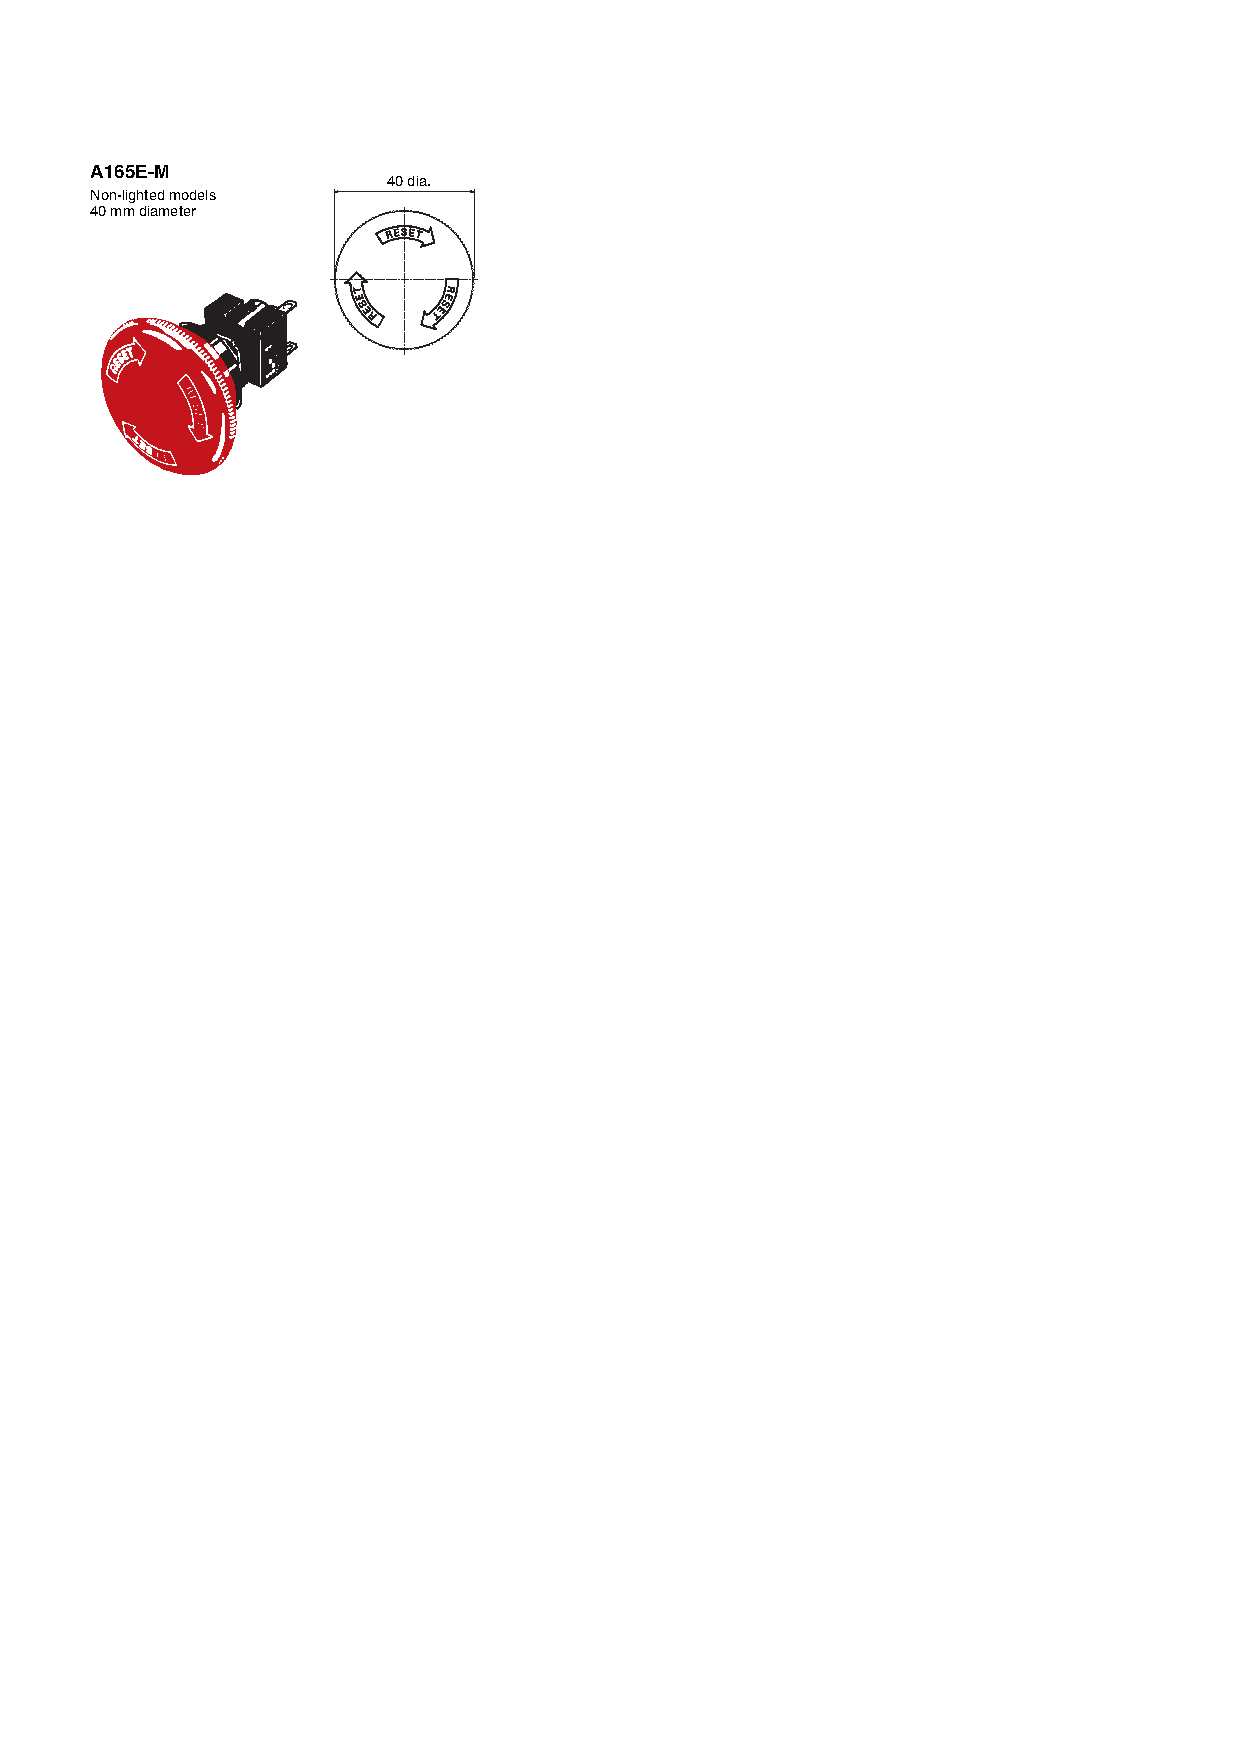
\includegraphics[width=.5\textwidth]{./img/SDC-A165E-M.pdf}
	\caption{Brake over travel switch.}
	\label{fig:SDC-A165E-M}
\end{figure}


\subsubsection{Wiring / additional circuitry}
\iffalse
Describe wiring and additional circuitry, show extra schematics for example if additional transistors etc. are used, also describe the function of additional circuitry and make good use of figures.
Additionally, fill out and add information to the following table:
\fi

If connector is used to connect SDC between control units, disconnecting any of them results in opening SDC and therefore opening AIRs as well. In other words the SDC directly carries the current driving the accumulator isolation relays(AIRs). All circuits that are part of the shutdown circuit have been designed in a way, that, when in disconnected state, they remove the current controlling the AIRs.

The cross-section of Shutdown System wire is AWG22. Block wiring scheme shown on \ref{fig:SDC-schematic}.\\

\begin{figure}[H]
	\centering
	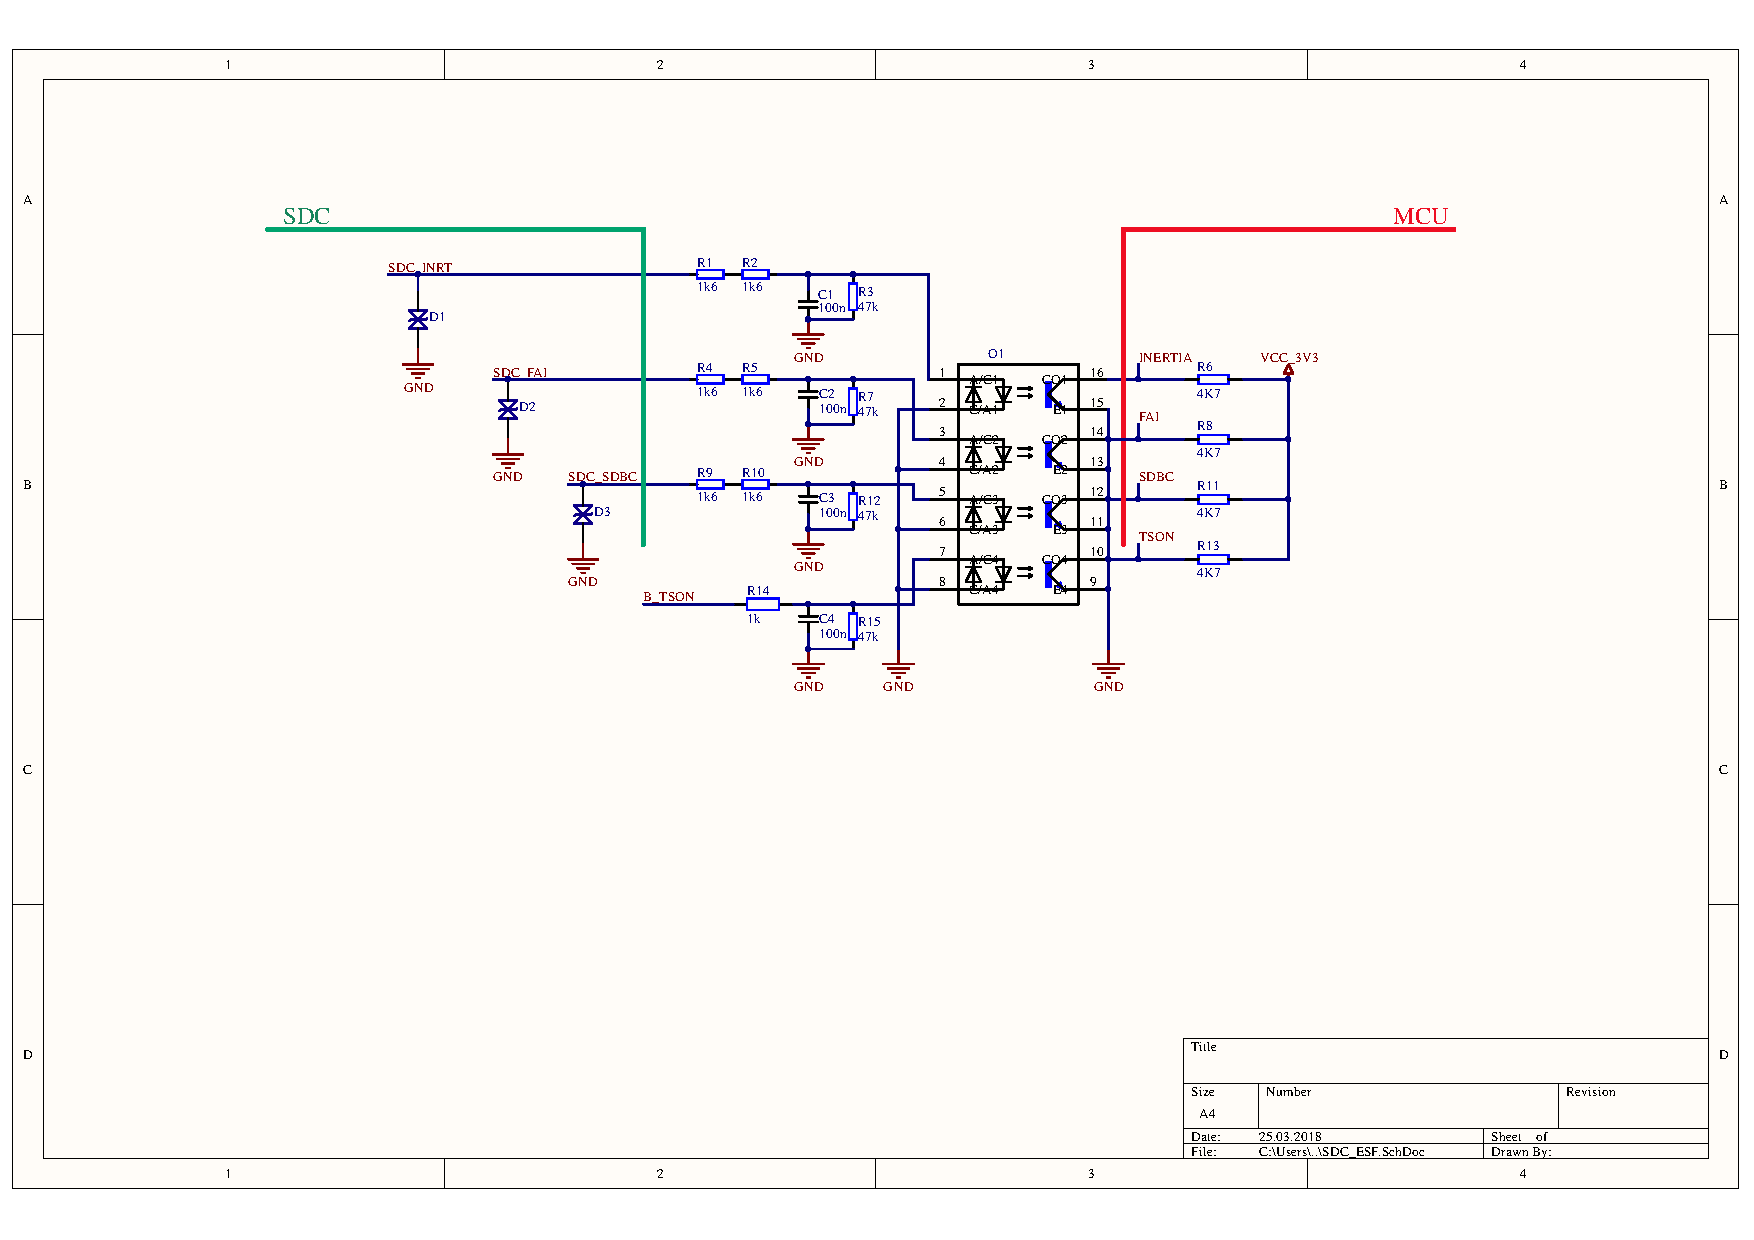
\includegraphics[width=\textwidth,trim={4cm 8cm 5cm 3cm}, clip]{./img/SDC-monitoring.pdf}
	\caption{Example of used SDC monitoring method with optocouplers.}
	\label{fig:SDC-schematic}
\end{figure}

As shown, 4k7 resistors are used to limit current through optocoupler. With 24V supply that makes 15,2mA per optocoupler. We used 8 optocouplers => 12*15, 2= 182,4mA.
% Table generated by Excel2LaTeX from sheet 'List1'
\begin{table}[H]
	\centering
	\caption{Wiring – Shutdown circuit}
	\begin{tabularx}{\textwidth}{|X|X|}
		\hline
		Total Number of AIRs: & 2 \\[\TableSize]
		\hline
		Current per AIR: & 70mA \\[\TableSize]
		\hline
		Additional parts consumption within the shutdown circuit: & 182,4mA \\[\TableSize]
		\hline
		Total current: & 322,4mA \\[\TableSize]
		\hline
		Cross sectional area of the wiring used: & 0,322mm2 (AWG22) \\[\TableSize]
		\hline
	\end{tabularx}%
	\label{tab:SDC-Wiring}%
\end{table}%


\subsubsection{Position in car}
\iffalse Provide CAD-renderings showing the relevant parts. Mark the parts in the renderings, if necessary. \fi
\begin{figure}[H]
	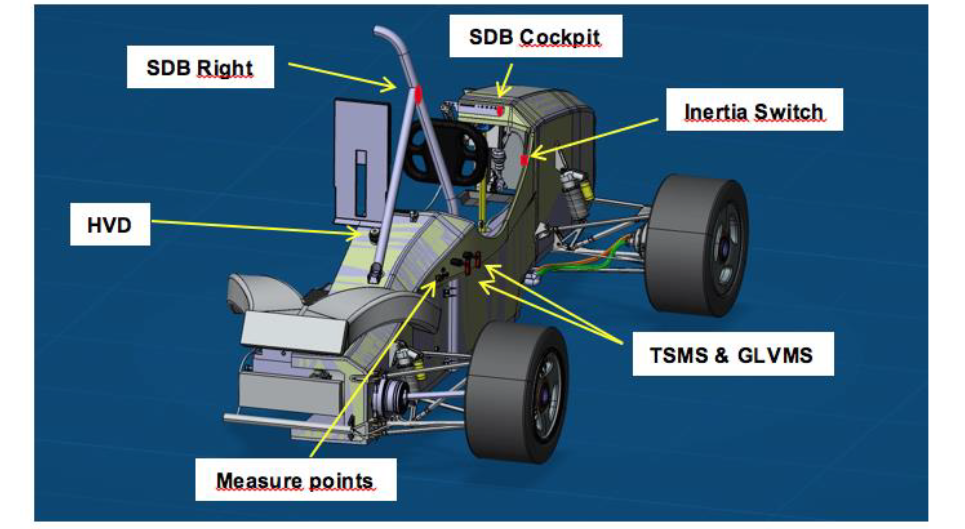
\includegraphics[width=\textwidth]{./img/SDC-positionInCar.png}
	\caption{Inertia switch, SDB Left, Right and Cockpit, TSMS, GLVMS, HVD, Measure points.}
	\label{fig:SDC-positionInCar}
\end{figure}